%!TEX root = thesis.tex

\chapter{Background}
\label{chap:literature}
    This chapter provides a discussion of the background and motivation of this work in further depth than the manuscripts presented later in this dissertation. Here, a general overview of ignitions as a threat to structures and fire spread and the current state of knowledge and predictive capabilities is communicated. Each manuscript includes a relevant and more detailed literature review pertaining to the specific objective of the chapter. 

\section{Widlfires and the WUI}
    Wildfires have been an integral part of many ecosystems for millennia and are often beneficial or required for maintaining a healthy ecosystem. As beneficial as they may be to the natural environment, wildfires pose a significant risk to the built environment. As communities around the world have expanded communities outward into environments that support wildfires (e.g., forests and grasslands), the risk of destruction of structures by wildfires has increased~\cite{Hammer2009DemographicManagement}. In the United States, 91\% of the Wildland Urban Interface (WUI) \nomenclature{WUI}{Wildland Urban Interface} growth of 189,000\si{\kilo\meter\squared} (larger than the state of Washington) development between 1990 and 2010 is occupied by homes~\cite{Radeloff2017} and has continued to grow on recent years. The increased development in these areas means that an excess of 40 million homes are located in areas that may be threatened by a wildfire. 
    
    In addition to the increase of homes in the WUI, the intensity and severity of fires have increased. California is an example of the increased fire severity where 13 of the 20 most destructive fires have occurred since 2010, and 7 of the 20 most destructive occurred in 2020 and 2021~\cite{CALFIRE2018}. Increasingly severe fires are not just limited to California. Texas and Tennessee each had one of the top ten most severe fires in the United States between 2005 and 2020. Colorado, Oregon, Washington, Oklahoma, and Florida have also seen highly destructive fires in recent years~\cite{Barrett2020}. The United States is not unique in the presence of wildfires that destroy homes. Australia's Black Summer in 2019-2020 was one of the most severe fire seasons in the country's history~\cite{Levin2021Unveiling2019/2020} where over 3000 homes and greater than 46 million acres burned~\cite{Filkov2020ImpactTrends}, which is approximately equivalent to 75\% of Oregon's land area. The Mediterranean countries of Portugal, Spain, France, Italy, and Greece are also either experiencing greater losses or are a risk for greater losses due to wildfires in recent years. Similar trends are also present in many Asian and South American countries~\cite{Manzello2018}. Wildfires that threaten lives, homes, and structures are truly a global phenomenon, and it is essential to understand how homes are ignited and destroyed in wildfires to better prevent losses from occurring.

\section{The Problem of Ignition}
    Ignition of a home in a WUI fire is attributed to three primary mechanisms; direct flame contact, ignition by radiative heating, and ignition by firebrands. Of these methods, ignition by firebrands is considered to be a primary threat to homes~\cite{Suzuki2021, Mell2010, Manzello2018FORUMResearch}. Case studies of WUI fires have consistently attributed structural losses to firebrand ignition~\cite{Westhaver2017WhyDisaster, Roberts2021} with one study attributing at least 2/3 of home losses to firebrands~\cite{Mell2011}. With the majority of ignitions occurring due to firebrand ignition, it is imperative to understand the mechanism of firebrand ignition to reduce home losses. An analysis of structures burned in California wildfires from 2013 to 2018 found that many of the homes lost would have been considered "fire-safe" by current standards but were still ignited by firebrands~\cite{Syphard2019}. Codes, standards, and best practices built upon a better understanding of ignition by firebrands would help provide better resilience to firebrand attacks~\cite{Manzello2020} reducing the number of homes lost in wildfires. Examples of these changes may include adjustments in building and landscaping materials favoring the selection of harder to ignite species or housing geometry constraints to reduce the collection of flammable materials or firebrands. Without a comprehensive knowledge of the ignition process, creating the codes and standards to reduce the risk of home loss is challenging at best and may even be counterproductive.  
    
    The general mechanism for firebrand ignition is considered to be a three-step process that starts within the fire itself, often at a significant distance from the ignition point. First, a firebrand is generated as burning material breaks off or is lofted into the air. Second, the firebrand is then lofted through the air and transported to the ignition site. Third, a firebrand lands on a recipient fuel bed, and then ignition occurs if the criteria for ignition are met~\cite{Babrauskas2003}. When considering the possibility of ignition during a fire event, all three processes must be considered as each process significantly influences the properties of a firebrand landing on a fuel bed. For example, the number, energy content, and size of firebrands that may land on a fuel bed are significantly influenced by the surrounding foliage~\cite{Hudson2020EffectsScale} and moisture content of the foliage~\cite{Adusumilli2021FirebrandShrub} which introduces significant variability in ignition sources a fuel bed may encounter. Similarly, the winds transporting a firebrand significantly influence the path of travel and time of flight, which influences the energy content~\cite{Sardoy2007, MatvienkoOVA2016} and localized winds around structures may lead to firebrand accumulation~\cite{Suzuki2020a, Suzuki2017a, Suzuki2015}. Unfortunately, the generation and ignition processes are significantly less understood than the transport processes~\cite{Manzello2020}. The work contained in this dissertation is focused on the ignition process of the fuel bed by a firebrand and does not consider the generation of firebrands. For further information on firebrand generation processes, the reader is referred to review papers considering this process by Fernandez-Pello~\cite{Fernandez-Pello2017}, Manzello et al.~\cite{Manzello2020} and Babrauskas~\cite{Babrauskas2003}.
    
    
    Firebrands have been identified as a source of structure loss as early as the 1600s~\cite{Suzuki2020} however, studies of firebrand ignition have only begun recently. Perhaps one of the first studies published to specifically address firebrands within the scope of structure loss was conducted by Waterman in 1969~\cite{Waterman1969ExperiemntalGeneration}. However, research remained sparse until the early 2000s. Early research and a significant portion of current research have been conducted by dropping combusting firebrands~\cite{Ellis2011, Ellis2015, Ganteaume2009, Manzello2006, Manzello2006a} (either flaming or glowing) or hot metal particles~\cite{Wang2017, Urban2017, Fernandez-Pello2015, Hadden2011} onto fuel beds in varying configurations that simulate conditions in a wildfire and observing ignition or no ignition outcomes. These works have identified some parameters that appear to control ignition but models created from these studies only provide qualitative predictions of ignition. The lack of models of quantitative accuracy was identified by Finney et al. in 2013, who identified the lack of a fundamental understanding of what processes occur and how they interact as a primary gap in the knowledge of ignition~\cite{Finney2013}. A similar need was identified by Manzello et al. in 2018~\cite{Manzello2018} and again in 2020~\cite{Manzello2020}. As fires increase in severity and the WUI continues to expand, the number of homes lost to wildfires is likely to increase in the near future significantly. Thus, the need for accurate predictions of ignition has never been higher. 
    
    
\section{Modeling Efforts}
    Creating a model with quantitative accuracy of ignition requires a thorough understanding of the processes and relative importance of each process leading up to ignition. Figure~\ref{fig:ignitionDiagram} illustrates the different factors that can influence the ignition process. To better understand how these parameters affect the ignition process can be considered as a series of three processes. The first is the heat transfer to the fuel bed from the firebrand. The second is the pyrolysis of the fuel bed material and the subsequent release of pyrolyzates into the air above the fuel bed. The third step is the mixing of the pyrolyzates with air above the fuel bed and subsequent gas-phase ignition. It is important to note that all three of these processes may occur simultaneously throughout the ignition process and are often interconnected. For example, as heat is transferred from the firebrand to the fuel bed, the thermal conductivity of the fuel bed changes with temperature both before and after pyrolysis begins~\cite{Fjellerup2003}. Furthermore, the heat transfer mode and thermal resistance between the firebrand and fuel continuously change as mass is released due to pyrolysis, which may influence ignition~\cite{Yang2016EffectParticle}. With the interconnection of the processes that occur during ignition and the inherent variability of fuel beds and biomass fuels in general, the quantification of parameters that influence ignition is quite challenging. Despite these challenges, results of previous research have identified influential parameters that have consistently been observed to control ignition. This work considers these parameters as belonging to one of three categories, namely, thermo-physical properties of the fuel bed, energy supplied by the firebrand, and environmental conditions near the ignition point. Detailed reviews of each category are provided in the relevant manuscripts and are not reproduced here. The remaining sections of this review address the predictive models of ignition that have been created from the current state of knowledge. The accuracy and applicability of each model are discussed in turn, and the remaining challenges are identified as they have motivated the objectives of this work. 
        \begin{figure}[hpbt]
            \centering
                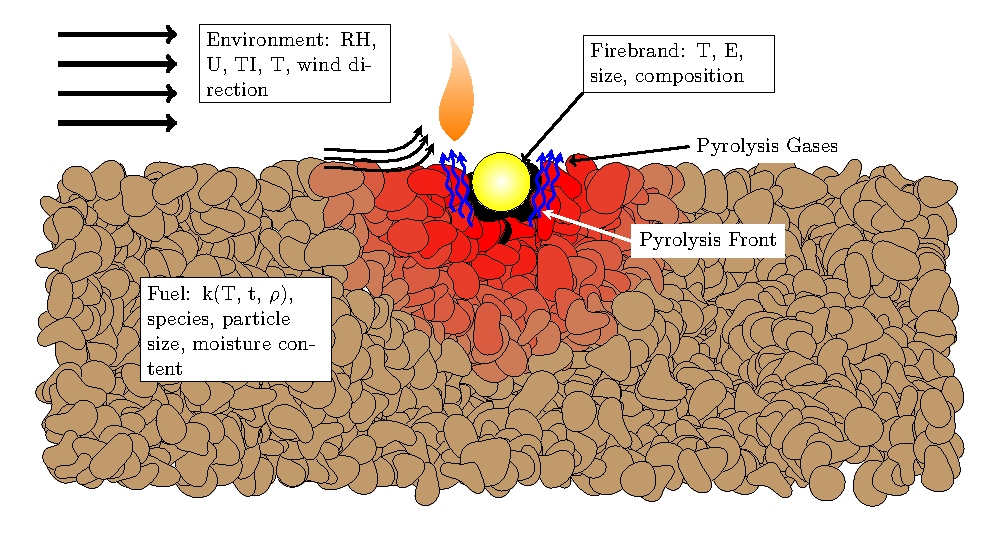
\includegraphics[width=\textwidth]{Figures/dissertationBed.pdf}
            \caption{Illustration of key features of fuel bed ignition and parameters/characteristics that may influence ignition. The black region near the firebrand represents char formed as the result of pyrolysis.}
            \label{fig:ignitionDiagram}
        \end{figure}
    
    Perhaps the first model to be considered for the ignition of wildland fuels is the hot spot theory. The hot spot model considers the ignition of a fuel bed by a heat source (firebrand) by determining the energy required for a thermally explosive reaction in the fuel~\cite{Zinn1962InitiationSpots, Thomas1965}. The minimum hot particle size for ignition of a fuel bed, as presented by Hadden et al.~\cite{Hadden2011}, is shown in Equation~\ref{eqn:hotspot}. 
    
        \begin{equation}
            r_{cr} = \delta_{cr}\sqrt{\frac{k}{\rho A \Delta H}\frac{RT^{2}_{p0}}{E} exp\left(\frac{E}{RT_{p0}}  \right)}
            \label{eqn:hotspot}
        \end{equation}
    In this equation, $\delta_{cr}$ is defined as the critical Frank-Kamenetskii hot spot parameter and is determined from calculations~\cite{Goldshleger1973IgnitionDimensions}. $\delta_{cr}$ is dependent on the ratio of volumetric heat capacities of the ignition source and the material, the activation energy of the material, and the temperature of the hot particle. In Equation~\ref{eqn:hotspot} $k, \rho A, E$, and $\Delta H$ are the thermal conductivity, density, pre-exponential factor, activation energy, and heat of combustion of the fuel bed material, respectively. $R$ is the universal gas constant, and $T_{p0}$ is the initial temperature of the heat source. Ultimately, Equation~\ref{eqn:hotspot} defines the particle energy needed to raise the temperature of a fuel bed region such that thermal runaway and subsequent ignition occurs. The hot spot theory has some limitations that prevent quantitative predictions of ignition in a wildfire setting. A discussion of the shortcomings of the hot spot theory is presented by Thomas~\cite{Thomas1965} and more recently presented by Hadden et al.~\cite{Hadden2011} with respect to wildfires. The two most significant shortcomings addressed by the previous works are neglecting heat losses to the surroundings and considering the pyrolysis and ignition phenomena as single-step, infinitely fast reactions. Hadden et al. attribute these shortcomings as a significant source of error for quantitative ignition predictions. This assertion is reinforced in a review by Fernandez-Pello~\cite{Fernandez-Pello2017} who concluded that in instances where hot spot theory has been applied, only qualitatively accurate predictions of ignition had been obtained. A similar model to hot spot theory but with a more comprehensive inclusion of heat loss from the firebrand was developed by Yin et al.~\cite{Yin2014}. A correlation between fuel properties, the energy transferred to the fuel bed, and the time to ignition was proposed and is shown in Equation~\ref{eqn:yinMC}.
        \begin{equation}
            \sqrt{t_{ig}} \approx \frac{q\sqrt{\frac{\rho_{f}k}{c_{p}}}}{\frac{\rho Z \Delta H_c}{t_b}- h_T(T_f - T_0)}
            \label{eqn:yinMC}
        \end{equation}
    Comparing the correlations presented in Equations~\ref{eqn:hotspot} and \ref{eqn:yinMC}, Equation~\ref{eqn:yinMC} includes properties of the fuel bed ($\rho$, $k$, $c_p$, $Z$, $T_0$) and  firebrand ($\rho_f$, $\Delta H_c/t_b$, $T_f$) as well as the energy required for ignition ($q$) mirroring the Frank-Kamenetskii critical hot spot diameter. The addition of heat losses to the ambient is the most significant difference from the hotspot parameter and addresses a key shortcoming of the hot spot theory. However, the model does not consider the combustion of the fuel bed other than the critical energy for ignition, leaving the second key gap for the hot spot theory unaddressed. Perhaps due to the omission of combustion, this model suffers a similar fate as the hot spot theory and follows qualitative trends but is not quantitative. Ultimately, the hot spot theory and similar models do not capture the complexity and variability inherent to ignition~\cite{Manzello2020}. 
    
    Another approach that has been used to predict the onset of ignition in fuels is defining the critical mass flux for ignition. The critical mass flux model asserts that if energy is transferred into a fuel bed at such a rate or quantity that the mass flux of pyrolysis products released is above the "critical" value, ignition will occur~\cite{Nelson1995}. The critical mass flux approach has been primarily considered for the ignition of solid materials such as PMMA~\cite{Rich2007} and wood slabs~\cite{Yashwanth2015, McAllister2013}. In these studies, the critical mass flux was well correlated with ignition; however, a general model that predicts ignition across materials and experiments is lacking. One shortcoming is the sensitivity to environmental conditions and material properties. In work conducted by McAllister for wooden plates, sensitivities to thermal boundary conditions were anticipated to be magnified in consideration of fuel beds made of particles. Differences in pyrolysis between the materials were also of concern as oxygen availability and boundary layer effects of the particle fuel beds were postulated to have a significant effect~\cite{McAllister2013}. Numerical studies considering the critical mass flux for a piloted ignition reported that the mass flux at ignition was sensitive to the Damkolher number above the fuel bed~\cite{Dai2013} giving further support to the sensitivity to boundary conditions (i.e., wind near the ignition source). While further study and development of the critical mass flux could potentially be expanded to address its shortcomings, other models have been developed that are more promising.
    
    Proposed ignition models that provide greater accuracy than the hot spot and critical mass flux models do so at the expense of complexity and computational cost. The majority of these models and modeling efforts use a two-part approach to join a pyrolysis-specific solver to address the chemical kinetics of an existing or custom computation fluid dynamics solver. This approach requires selecting a combination of three parts, each of which has limitations and considerations which may affect the accuracy of ignition predictions. First, an appropriate chemical kinetic mechanism must be chosen based on the computational resources available. For example, many early works~\cite{DiBlasi1996} and some more recently~\cite{Ding2015, Torero2020} have considered pyrolysis to occur as a single step process or as a process of few reactions (approximately ten or fewer). Newer kinetic mechanisms have been developed to more completely capture the processes of pyrolysis and are much more complex. Perhaps the most comprehensive mechanisms are extended forms of the mechanism developed by Ranzi et al.~\cite{Ranzi2008}. Additions to this mechanism have expanded the method to include extractives to cover a greater variety of biomass~\cite{Debiagi2015} and the addition of reactions to address gas-phase reactions previously not considered~\cite{Dhahak2019}. For a more detailed discussion of the progression and challenges of biomass pyrolysis, the reader is referred to review articles by Di Blasi~\cite{DIBLASI199371} and more recently by Haberle et al.~\cite{Haberle2017}. 
    
   One of the most recent and most promising tools for ignition modeling and pyrolysis is Gpyro which is a pyrolysis solver specifically designed to handle both the condensed (solid) and gas phase of biomass combustion~\cite{Lautenberger2009a}. Gpyro is often coupled with the Fire Dynamics Simulator (FDS)~\cite{FDSManual}, an LES solver specifically designed to capture physics relevant to fires, to form a complete computational package. The combination of Gpyro and FDS has been utilized to observe combustion sensitivities and ignition sensitivities. For example, a study of the effects of moisture content on ignition using Gpyro/FDS suggested that moisture in the fuel affected ignition, gas-phase combustion, and pyrolysis of the fuel~\cite{Yashwanth2016}. Other studies using Gpyro/FDS have been conducted to predict ignition and observe controlling parameters~\cite{Shotorban2018, Fernandez-Pello2015, Lautenberger2009}. Unfortunately, the Gpyro/FDS modeling requires significant computational expenditure. The high computational cost of tools like Gpyro/FDS prevents them from practical application across the vast number of configurations and possible ignition threats present in the wildland urban interface.
    
    To balance the need for accuracy and computational cost, a usable and accurate model is anticipated to be between the critical mass flux and the full CFD model with respect to complexity. The understanding of the effects (e.g., environmental conditions, fuel bed properties.) that are most influential to ignition is not complete enough to develop such a model. Bridging this knowledge gap by identifying and quantifying which parameters are the most influential to ignition or non-ignition outcome is the overall goal of this work. The identification of the most influential parameters is anticipated to enable the creation of a model that can predict ignition across a variety of fuel beds, firebrands, and environmental configurations.
